\setcounter{chapter}{1}\chapter{Knowledge and Data}
\begin{exsol@solution}{1.6-1}
1.  What might be wrong about these headlines?
  a.	A study proclaims: ``Slightly overweight people live longer than thin people.'' ``Slightly overweight people live longer than thin people.''  It is a fallacy of correlation equals causation.  It statement implies that being slightly overweight causes people to live longer when compared to thin people.  We would want to dig deeper into the study to see what confounding variables may be present: did we take into account health of the individuals?  Perhaps we have some individuals in poor health leading them to be thin and shortening their lives.

\end{exsol@solution}
\begin{exsol@solution}{1.6-3}
No randomization; the product was given to several people; a skin specialist should make the determination as to the effectiveness of the product; the company should not mass produce this anti-wrinkle cream.

\end{exsol@solution}
\setcounter{chapter}{2}\chapter{Data Presentation}
\begin{exsol@solution}{2.8-1}
    \begin{enumerate}
	  \item   numeric, ratio
    \item  categorical, nominal
    \item  numeric, ratio
    \item  categorical, nominal
    \item  numeric, interval
    \item  categorical, ordinal
    \item  categorical, ordinal
    \item  categorical, ordinal
    \item  numeric: ratio
    \item  categorical, ordinal
    \item  categorical, nominal
    \item  categorical, ordinal
    \item  numeric, interval
  	\end{enumerate}
\end{exsol@solution}
\begin{exsol@solution}{2.8-2}

\end{exsol@solution}
\begin{exsol@solution}{2.8-3}

Compute relative frequencies:

\begin{tabular}{@{} lcc @{}} \hline
Interval  &  Frequency &	Relative Frequency \\
$(20, 25]$ 	&     4 & 4  \\
$(25, 30]$ 	&    11 & 11 \\
$(30, 35]$ 	&    23 & 23 \\
$(35, 40]$ 	&    31 & 31 \\
$(40, 45]$ 	&    15 & 15 \\
$(45, 50]$ 	&    10 & 10 \\
$(50, 55]$ 	&     6 & 6 \\ \hline
\end{tabular}


\end{exsol@solution}
\begin{exsol@solution}{2.8-4}
2.5-7.1: Left-skewed

2.5-7.2: Symmetric

2.5-7.3: Left-skewed

2.5-7.4: Right-skewed

2.5-7.5: Symmetric

\end{exsol@solution}
\begin{exsol@solution}{2.8-5}
	  The level of measurement of marital status is nominal.
\end{exsol@solution}
\begin{exsol@solution}{2.8-6}
	  The level of measurement of marital status is category - nominal.
\end{exsol@solution}
\begin{exsol@solution}{2.8-7}
	  The number of reported robberies in June 2014 is Kalamazoo County is a continuous variable.
\end{exsol@solution}
\begin{exsol@solution}{2.8-8}

    Numeric - interval

\end{exsol@solution}
\begin{exsol@solution}{2.8-9}
    Numeric - ratio
\end{exsol@solution}
\begin{exsol@solution}{2.8-10}
    all adult residents of the U.S.
\end{exsol@solution}
\begin{exsol@solution}{2.8-11}
    birth weight.
\end{exsol@solution}
\begin{exsol@solution}{2.8-12}

    Variable: Homicide rate \\
    Level of Measurement: Interval-ratio \\
    Type: Continuous \\
    Application: Descriptive (two variables)

\end{exsol@solution}
\begin{exsol@solution}{2.8-13}

    Variable: party, gender, opinion \\
    Level of Measurement: nominal, nominal, ordinal \\
    Type: discrete, discrete, discrete \\
    Application: inferential, NA, NA

\end{exsol@solution}
\begin{exsol@solution}{2.8-14}
    All of the choices is the correct answer.
\end{exsol@solution}
\setcounter{chapter}{3}\chapter{Location and Spread}
\begin{exsol@solution}{3.4-1}

	Compute the mean, median, $\dots$ for carbon monoxide:
  \begin{enumerate}
  \item mean = 12.5
  \item median = 13.0
  \item Trimmed mean = 12.7
  \item SD = 4.74
  \item Mean = 0.0125 and standard deviation 0.00474 (in grams)
\end{exsol@solution}
\begin{exsol@solution}{3.4-3}


\begin{enumerate}
\item The range is from 13 to 59
\item the mean is 46.7
\item The median is 49.5
\item There is no mode since there are no duplicates.
\item Removing the smallest value changes the mean to 50.4.  The new value is closer to median because 13 is an outlier.
\end{enumerate}
\end{exsol@solution}
\begin{exsol@solution}{3.4-4}

% \begin{enumerate}
% \item the mean is mn1
% \item the median is md1
% \item Decide if its symmetric, skewed to the right or to the left: the data is right skewed
% \item Decide which measure of center provides the most relevant information about the distribution? Why?  The median is the most relevant information because the data is right skewed.
% \end{enumerate}

\end{exsol@solution}
\begin{exsol@solution}{3.4-5}

\begin{enumerate}
\item $\bar{x} = 262.2$
\item $\tilde{x} = 197$
\item $sd = 245.6360451 $
\item The distribution is Right skewed
\item The median provided the most relevant information because to the extreme outlier.
\end{enumerate}

\end{exsol@solution}
\begin{exsol@solution}{3.4-6}
	
	Compute the mean, median, and mode for the weekly grocery budget
	mean = 32.167, median = 32.5, mode = 35
	
\end{exsol@solution}
\begin{exsol@solution}{3.4-7}
	
	The third value must be 22 so that the average is 20 for all three quizzes.
	
\end{exsol@solution}
\begin{exsol@solution}{3.4-8}




    The mean is 472.59875
    The median is 555
    There is no mode since there are no duplicates.

{\bf{1. }} The greater value is the median (555).  {\bf{2. }} There is a negative skewness in the middle half the of the dataset.  (Refer to Figure 3.1.)

\begin{figure}[htbp] %  figure placement: here, top, bottom, or page
   \centering
   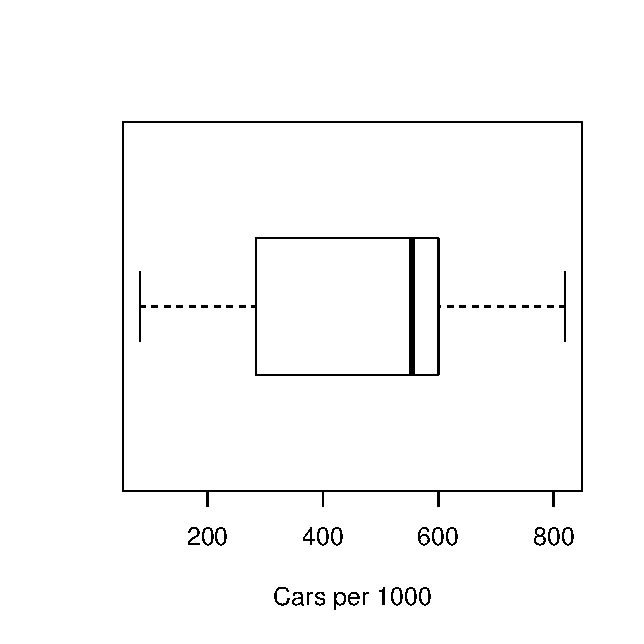
\includegraphics[width=6cm]{figure/f3_1-1.pdf}
   \caption{Boxplot of Cars per 1000}
   \label{fig:f3_1}
\end{figure}

{\bf{3. }} When we compare the median to the mean, we find the median (555) is greater the mean (472.6).  Therefore, we can say the the dataset is left skewed.

\end{exsol@solution}
\begin{exsol@solution}{3.4-9}

  {\bf{(1. )}} Mode  {\bf{(2. )}} Median  {\bf{(3. )}} Mean  {\bf{(4. )}} Mean  {\bf{(5. )}} Median  {\bf{(6. )}} Mode

\end{exsol@solution}
\begin{exsol@solution}{3.4-10}
    {\bf{Birth}} Mode=``North'';   {\bf{Expense}} Mean=48.5; {\bf{Movies}} Mean=5.8; {\bf{Food}} Median=6;  {\bf{Religion}} Mode=``Protestant''

\end{exsol@solution}
\begin{exsol@solution}{3.4-11}



The mean for 2005 is 55.4.
The median for 2005 is 54.5.
The mean for 2015 is 57.1.
The median for 2015 is 57.

\end{exsol@solution}
\begin{exsol@solution}{3.4-12}

	The mean is
[1] 31.8


	The median is
[1] 35


\end{exsol@solution}
\begin{exsol@solution}{3.4-13}




  The mean is 28.72, and the median is 30

\end{exsol@solution}
\begin{exsol@solution}{3.4-14}




	The pretest mean is  9.3333333


	The pretest median is 10


	The posttest mean is	12.9333333


The pretest median is 12


\end{exsol@solution}
\setcounter{chapter}{4}\chapter{Threats to Valid Comparisons}
\begin{exsol@solution}{4.4-1}
	  $H_0: \mu = 6.2$ vs. $H_A: \mu \neq 6.2$
\end{exsol@solution}
\begin{exsol@solution}{4.4-3}

    From the distribution of $t$, using row df = 24 and column 0.025, CV(t) = 2.064.
\end{exsol@solution}
\setcounter{chapter}{5}\chapter{Study Designs}
\begin{exsol@solution}{5.5-2}
Randomized controlled experiments are necessary to establish the cause of such a disease firmly. For instance, we might see if potassium deficiency causes the disease, we may give our treatment group a potassium supplement every day. However, if the illness is rare, then it is impractical for us to use a randomized controlled experiment.  It would also be unethical to be influencing or causing disease in people potentially.  Additionally, we would have no guarantee that any subjects would even develop the disease if it is sporadic. Thus, observational studies may be the most appropriate choice unless scientific advances in, say, genetics are far enough along to make a more practical kind of randomized controlled experiment.
	
\end{exsol@solution}
\begin{exsol@solution}{5.5-4}
A randomized controlled experiment is the ``gold standard of scientific knowledge'' so that it would be the best way to study this situation. We would study four groups of patients: group one would get a standard treatment for an illness, group two would get a placebo without being told it's a placebo, group 3 would get a placebo and told it's a placebo, and group 4 would get no treatment at all. This method would, interestingly, give controls both from the standard and no-treatment groups. The groups for primary comparisons would be the two groups that get the placebos and are either informed or not.

\end{exsol@solution}
\begin{exsol@solution}{5.5-6}
Yes, there are potential confounders. For instance, it might be that players feel better rested at the start of a game, so they play harder and get injured more frequently because of this possibility. The organization could investigate the frequency of injuries that occur during later kickoffs in the game or to conduct small-scale randomized controlled experiments that change kickoff rules before recommending substantial sweeping changes.

\end{exsol@solution}
\setcounter{chapter}{6}\chapter{The Normal Distribution}
\begin{exsol@solution}{6.7-1}

\begin{enumerate}
	\item The proportion of cell phone users are on their phones between 1 hour
and 3 hours per day is 0.6057221
  \item Just to be safe, suppose you decide to be in the 5th percentile of
cell phone users in terms of monthly usage.  How much time can you spend on your phone per day? You decide to spend no more than 35.4396606 minutes on your phone per day.
	\end{enumerate}
\end{exsol@solution}
\begin{exsol@solution}{6.7-3}


    The standard deviation is $SD = \frac{35 - 4}{4} = 7.75$
\end{exsol@solution}
\begin{exsol@solution}{6.7-5}

\begin{enumerate}
\item The probability that the stock price is between 39.88 and 46.01 is $P[39.88 < X < 46.01] = 0.9395927$.
\item The probability that the stock price is above 40 is $P[X > 40] = 0.9327388$.
\item The probability that the stock price is below 40 si $P[ x < 40] = 0.0672612$.
\end{enumerate}
\end{exsol@solution}
\begin{exsol@solution}{6.7-7}
\begin{enumerate}
\item The area to the left of 0.0 is.5000
\item The area to the left of 0.2 is.5793
\item The area to the left of 0.25 is.5987
\item The area to the left of 2.25 is.9878
\end{enumerate}
\end{exsol@solution}
\begin{exsol@solution}{6.7-8}
	  \begin{equation}
	    SD = \frac{(41 - 32)}{3} = 3
	  \end{equation}
\end{exsol@solution}
\begin{exsol@solution}{6.7-9}
	  \begin{equation}
	    z = \frac{173 - 153}{11} = 1.82
	  \end{equation}
\end{exsol@solution}
\begin{exsol@solution}{6.7-10}

	    $z = \frac{143 - 155}{12} = -1$ \\
	    $P[z < -1] = 15.87$

\end{exsol@solution}
\begin{exsol@solution}{6.7-11}

	    $x = \mu + Z \sigma$ \\
	    $x = 155 + 1.28 \times (12) $ \\
	    $x = 170.36$

\end{exsol@solution}
\begin{exsol@solution}{6.7-12}

	    $x = \mu + Z \sigma$ \\
	    $x = 155 - 0.6745 \times (12) $ \\
	    $x = 146.91$

\end{exsol@solution}
\begin{exsol@solution}{6.7-13}



	  The value of the $15^{th}$ percentile is 4.9585388.

	  There are six countries: Congo (4.1), Indonesia (3.1), Saudi Arabia (3.2), Venezuela (3.6), India (4.0), Malaysia (4.0), and Thailand (4.6).

\end{exsol@solution}
\begin{exsol@solution}{6.7-14}



    The probability of having a mean less than 7.3 ($P[ \bar{x} < 7.3 ]$) is 0.3782144.

\end{exsol@solution}
\begin{exsol@solution}{6.7-15}



    The probability of having a mean greater than 9.3 ($P[ \bar{x} > 9.3 ]$) is 0.6217856.

\end{exsol@solution}
\begin{exsol@solution}{6.7-16}



    The probability of having a mean between 7.3 and  9.3 ($P[ 7.3 < \bar{x} < 9.3 ]$) is 0.2435711.

\end{exsol@solution}
\setcounter{chapter}{7}\chapter{The Binomial Distribution}
\begin{exsol@solution}{7.8-1}

		\begin{enumerate}
	  \item The mean and standard deviation are 5 and 1.5811388, respectively.
    \item The probability that there are more than 5 successes is $P[ X > 5 ] = 0.3769531$.
    \item The probability that there are fewer than 5 successes is $P[ X < 5 ] = 0.3769531$.
    \item The probability that there  are between 1 and 3 successes  is $P[ 1 \le X \le 5 ] = 0.1708984$.
	  \end{enumerate}
\end{exsol@solution}
\begin{exsol@solution}{7.8-3}

\begin{enumerate}
\item The probability that at least 100 people are Apple users is $P[X \ge 100] = 0.3070581$.
\item The probability that at most 100 people are Apple users is $P[X \le 100] = 0.7302684$.
\item The probability that between 80 and \\ 120 people are Apple users is $P[ 80 \le X \le 120] = 0.9572505$.
\end{enumerate}
\end{exsol@solution}
\begin{exsol@solution}{7.8-5}

\begin{enumerate}
\item The probability that he gets at least 7 hits is $P[X \ge 7] = 0.0048184$.
\item The probability that he gets at most 1 hit is $P[X \le 1] = 0.1461307$.
\item The probability that he gets between 4 and 6 hits is $P[4 \le X \le 6] = 0.3245785$.
\end{enumerate}

\end{exsol@solution}
\begin{exsol@solution}{7.8-7}

The expected value is 8 and SD is 2.7712813
\end{exsol@solution}
\begin{exsol@solution}{7.8-8}



\begin{enumerate}
\item $P[ x \ge 33] = 0.2352$
\item $P[ x \le 25] = 0.0970$
\end{enumerate}

\end{exsol@solution}
\setcounter{chapter}{8}\chapter{Sampling Distribution of the Proportion}
\begin{exsol@solution}{8.7-1}

$P[ X \ge 32 ] = 0.0760321
\end{exsol@solution}
\begin{exsol@solution}{8.7-3}

The standard error of this estimate is 0.04

\end{exsol@solution}
\begin{exsol@solution}{8.7-5}

\begin{enumerate}
\item	The estimate of the population proportion is \\ $\hat{p} = 0.2583333$
\item	The standard error of this estimate is \\ $SE_{\hat{p}} = 0.039958$
\item	The 95\% confidence interval is \\ $0.2583333 \pm 0.0783177$
\end{enumerate}
\end{exsol@solution}
\begin{exsol@solution}{8.7-7}

\begin{enumerate}
\item	The estimate of the population proportion is \\ $\hat{p} = 0.3$
\item	The standard error of this estimate is \\ $SE_{\hat{p}} = 0.010247$
\item The margin of error the estimate is \\ $M_{\hat{p}} = 0.020084$
\item	The 95\% confidence interval is \\ $0.3 \pm 0.020084$
\item	The 95\% confidence interval is \\ $0.3 \pm 0.020084$
\end{enumerate}
\end{exsol@solution}
\begin{exsol@solution}{8.7-8}

The standard error of this estimate is 97

\end{exsol@solution}
\setcounter{chapter}{9}\chapter{Comparing Two Proportions }
\begin{exsol@solution}{9.5-1}


\begin{enumerate}
\item The difference in the percentage of drug use \\ between smokers and nonsmokers is 35.0.
\item Calculate a standard error for our estimate in (1).
\item Calculate a 95\% confidence interval for the difference in the percentage of drug use \\ between smokers and nonsmokers.
\item Estimate the risk ratio of drug use \\ between smokers and nonsmokers.
\item Calculate a standard error for the natural log of our estimate in 4.
\item Calculate a 95\% confidence interval for the risk ratio of drug use between smokers
\item Estimate the odds ratio of drug use \\ between smokers and nonsmokers.
\item Calculate a standard error for the natural log of our estimate in 7.
\item Calculate a 95\% confidence interval for the odds ratio of drug use between smokers and nonsmokers.
\item Interpret the above confidence intervals in parts 3, 6, and 9. Which are significant, and which are not? Why or why not?
\end{enumerate}

\end{exsol@solution}
\begin{exsol@solution}{9.5-3}
   The critical value is


  1.984217

\end{exsol@solution}
\begin{exsol@solution}{9.5-5}
	

	
	  \begin{enumerate}
	  \item Conclude that there is a difference since zero is not within the interval that the difference in the proportion of men and women who think that it is wrong for married people to have an affair.
	  \item SE = 0.0243
	  \item RR = 1.0581245
	  \item OR = 1.5752837
	  \end{enumerate}	
	
\end{exsol@solution}
\setcounter{chapter}{10}\chapter{Sampling Distribution of the Mean}
\begin{exsol@solution}{10.7-1}
\end{exsol@solution}
\begin{exsol@solution}{10.7-2}
\begin{enumerate}
  \item The standard error of this estimate is $SE = \frac{2}{\sqrt{16}} = 0.5$
  \item The 95\% margin of error is $ME = 1.96 \times SE = 1.96 \times 0.5 = 0.98$
  \item The 95\% CI is $\bar{x} \pm ME = 10.5 \pm 0.98 = (9.52, 11.48) $
  \item
  \begin{eqnarray*}
      P[ \bar{x} > \mu ] &=& P[z > z^*] \\
       P[z > z^*] &=& P\Big[ z > \frac{ \bar{x}-\mu}{ \sigma/\sqrt{n}} \Big] \\
       &=& P\Big[ \frac{z > 9 - 10}{ 2/\sqrt{16}} \Big] \\
       &=& P\Big[ z > \frac{-1}{0.5} \Big]   \\
        &=& P[z > -2]
        &=& 1 - 0.025 = 0.975
  \end{eqnarray*}

  \item
  \begin{eqnarray*}
      P[ \bar{x} < \mu ] &=& P[z < z^*] \\
       P[z < z^*] &=& P\Big[ z < \frac{ \bar{x}-\mu}{ \sigma/\sqrt{n}} \Big] \\
       &=& P\Big[ z < \frac{ 9 - 10}{ 2/\sqrt{16}} \Big] \\
       &=& P\Big[ z < \frac{-1}{0.5} \Big]   \\
        &=& P[z < -2]
        &=&  0.025
  \end{eqnarray*}

  \item
  \begin{eqnarray*}
      P[ 8 < \bar{x} < 10 ] &=& P[ z^* < z < z^{**} ] \\
       P[z < z^*] &=& P\Big[ z < \frac{ \bar{x}-\mu}{ \sigma/\sqrt{n}} \Big] \\
       &=& P\Big[ z < \frac{ 8 - 10}{ 2/\sqrt{16}} \Big] \\
       &=& P\Big[ z < \frac{-2}{0.5} \Big]   \\
        &=& P[z < -4] \\
        P[z < z^*] &=& P\Big[ z < \frac{ \bar{x}-\mu}{ \sigma/\sqrt{n}} \Big] \\
       &=& P\Big[ z < \frac{ 10 - 10}{ 2/\sqrt{16}} \Big] \\
       &=& P\Big[ z < \frac{-2}{0.5} \Big]   \\
        &=& P[z < 0]
      P[ z^* < z < z^{**} ] &=& P[ -4 < z < 0] \\
        &=&  P[ z < 0 ] - P[z < -4] \approx 0.5 - 0 \\
        &=& 0.5
  \end{eqnarray*}



  \item 33\% of sample means are above what value?
  \item 33\% of sample means are below what value?
\end{enumerate}
\end{exsol@solution}
\begin{exsol@solution}{10.7-3}
\end{exsol@solution}
\begin{exsol@solution}{10.7-4}
\end{exsol@solution}
\begin{exsol@solution}{10.7-5}
\end{exsol@solution}
\begin{exsol@solution}{10.7-6}
\end{exsol@solution}
\setcounter{chapter}{11}\chapter{Comparing Two Means}
\begin{exsol@solution}{11.5-1}

\end{exsol@solution}
\begin{exsol@solution}{11.5-2}
\end{exsol@solution}
\begin{exsol@solution}{11.5-3}
\end{exsol@solution}
\begin{exsol@solution}{11.5-4}

\end{exsol@solution}
\begin{exsol@solution}{11.5-5}
\end{exsol@solution}
\begin{exsol@solution}{11.5-6}
\end{exsol@solution}
\begin{exsol@solution}{11.5-7}


\begin{enumerate}
  \item $\bar{X}_d = 0.4 $
  \item $SE_d = 0.4$
  \item $95\% CI  \rightarrow ( -0.4525798, 1.2525798 )$
  \item Does the data support the claim that the new material gives superior wear?  No, since zero is contained in the 95\% CI.
\end{enumerate}

\end{exsol@solution}
\setcounter{chapter}{12}\chapter{Categorical Variables: Association or Independence}
\begin{exsol@solution}{12.4-1}
\end{exsol@solution}
\begin{exsol@solution}{12.4-2}
\end{exsol@solution}
\begin{exsol@solution}{12.4-3}
\end{exsol@solution}
\begin{exsol@solution}{12.4-4}
\end{exsol@solution}
\begin{exsol@solution}{12.4-5}
\end{exsol@solution}
\setcounter{chapter}{13}\chapter{Correlation}
\begin{exsol@solution}{13.4-1}


13.5-1.1: $r = 0.9527 $

13.5-1.2: same, $r = 0.9527 $

13.5-1.3: same, $r = 0.9527 $

13.5-1.4: same, $r = 0.9527 $

13.5-1.5: same but the sign changed, $r = -0.9527 $

\end{exsol@solution}
\begin{exsol@solution}{13.4-2}
$r = 1$ because the points (x, y) all fall perfectly along a line tilted upward.

\end{exsol@solution}
\begin{exsol@solution}{13.4-3}
\end{exsol@solution}
\begin{exsol@solution}{13.4-4}

\end{exsol@solution}
\begin{exsol@solution}{13.4-5}
$ -1 < r < 0$. We know $r$ is negative because the line of best fit is tilted downward. We know $r$ is not $-1$ nor $0$ because the points are clustered, but do not perfectly fall on, the line of best fit.

\end{exsol@solution}
\begin{exsol@solution}{13.4-6}
\end{exsol@solution}
\begin{exsol@solution}{13.4-7}
Since $ r = \frac{ \sum Z_x Z_y}{(n - 1)}$, and we know that all the products of Z scores are negative, we know that r must be -1≤r<0. Since $ r = \frac{ \sum Z_x Z_y}{(n - 1)}$, and we know that all the products of Z scores are negative, we know that $r$ must be $-1 \le r < 0$.
\end{exsol@solution}
\setcounter{chapter}{14}\chapter{Linear Regression}
\begin{exsol@solution}{14.7-1}
\begin{enumerate}
  \item Calculate the regression line for predicting Y from X.
  \item Draw the scatterplot with an overlaid regression line.
  \item Add 5 to Y, so the new values are 5, 8, 15, 6, 20.  Calculate the new regression line.
  \item Multiply Y by 5, so the new values are 0, 15, 50, 5, 75.  Calculate the new regression line.
\end{enumerate}

\end{exsol@solution}
\begin{exsol@solution}{14.7-2}
\end{exsol@solution}
\begin{exsol@solution}{14.7-3}

\end{exsol@solution}
\begin{exsol@solution}{14.7-4}
     $ BAC = -0.012 + 0.017 (9) = 0.14 $
\end{exsol@solution}
\begin{exsol@solution}{14.7-5}
    A moderately strong positive straight-line relationship between number of beers and BAC.
\end{exsol@solution}
\begin{exsol@solution}{14.7-6}
       The correllation coefficient is $r = 0.875 = \sqrt{0.765}$ where  $r^2$ is the coefficient of determination.
\end{exsol@solution}
\begin{exsol@solution}{14.7-7}
       The independent variable is HEIGHT and the dependent variable is rincom06.
\end{exsol@solution}
\begin{exsol@solution}{14.7-8}

       $H_0: \beta = 0" vs. $H_1: \beta \ne 0$

\end{exsol@solution}
\begin{exsol@solution}{14.7-9}

       The correlation coefficient between the respondent's height and income is 0.0363929

\end{exsol@solution}
\begin{exsol@solution}{14.7-10}

       \begin{table}[ht]
    \centering
    \begin{tabular}{lr} \hline
        &  \multicolumn{1}{c}{Independent} \\ \hline

    Dep. Var. & 1. height      \\ \hline
    1. income  &   0.1907692      \\ \hline

    \end{tabular}
    \end{table}


\end{exsol@solution}
\begin{exsol@solution}{14.7-11}

    For a sample of 40 subjects, we tested the relationship between height and income.  We found a weak positive relationship using the correlation coefficient (0.1907692).  We then looked at the slope:  as {\textit{height}} increases by one inch, {\textit{income}} increases by 0.2777942 with a p-value of


\end{exsol@solution}
\begin{exsol@solution}{14.7-12}
       The independent variable is income,   age, and absingle and the dependent variable is happiness.
\end{exsol@solution}
\begin{exsol@solution}{14.7-13}

       $H_0: \beta_1 = \beta_2 = \beta_3 = 0$ \\
       $H_1:$ at least one slope is not equal zero. \\
       where $\beta_1$ is the slope for Happiness and Income,  $\beta_2$ is the slope for Happiness and Age and $\beta_3$ is         the slope for Happiness and single.

\end{exsol@solution}
\begin{exsol@solution}{14.7-14}

       Read the results from the computer generated output.

\end{exsol@solution}
\begin{exsol@solution}{14.7-15}

      The results are in the table.

\end{exsol@solution}
\begin{exsol@solution}{14.7-16}

  The results are in the table.

\end{exsol@solution}
\begin{exsol@solution}{14.7-17}
       The independent variable is income,   age, and absingle and the dependent variable is happiness.
\end{exsol@solution}
\begin{exsol@solution}{14.7-18}

       $H_0: \beta_1 = \beta_2 = \beta_3 = 0$ \\
       $H_1:$ at least one slope is not equal zero. \\
       where $\beta_1$ is the slope for Happiness and Income,  $\beta_2$ is the slope for Happiness and Age and $\beta_3$ is         the slope for Happiness and single.

\end{exsol@solution}
\begin{exsol@solution}{14.7-19}

       Read the results from the computer generated output.

\end{exsol@solution}
\begin{exsol@solution}{14.7-20}

      The results are in the table.

\end{exsol@solution}
\begin{exsol@solution}{14.7-21}

  The results are in the table.


\end{exsol@solution}
\setcounter{chapter}{15}\chapter{Workshops}
\begin{exsol@solution}{15.-1}

  \begin{enumerate}
  \item Construct a relative frequency table for total student majors (column above).
  \item	The highest percentage of students fall under what major?
  \item	What percentage of students are Art majors?
  \item	What percentage of students’ majors fall in both Sociology and Psychology?
  \item	How does the percentage of students who are communications majors in Class A compare to the percentage of communication majors overall for total students?
\end{enumerate}
\end{exsol@solution}
\begin{exsol@solution}{15.-2}
  \begin{enumerate}
  \item	Using the column `RF' above, construct a relative frequency table for student majors in the Web Class only.
  \item	The highest percentage of students fall under what major?
  \item	What percentage of students are Music majors?
  \item	What percentage of students are found in the majors of Psychology, Social Work and Sociology (combined)?
  \item	How does the percentage of students who are education majors in the Web class compare to the percentage of education majors overall for total students?  Which is higher?
\end{enumerate}
\end{exsol@solution}
\begin{exsol@solution}{15.-3}
  \begin{enumerate}
  \item	Using the column `RF' above, construct a relative frequency table for student majors in the Web Class only.
  \item	The highest percentage of students fall under what major?
  \item	What percentage of students are Music majors?
  \item	What percentage of students are found in the majors of Psychology, Social Work and Sociology (combined)?
  \item	How does the percentage of students who are education majors in the Web class compare to the percentage of education majors overall for total students?  Which is higher?
\end{enumerate}
\end{exsol@solution}
\begin{exsol@solution}{15.-4}
  \begin{enumerate}
  \item Fill in the frequency and relative frequency table above
  \item  Create a bar chart and pie chart for the above data
  \item  What percentage of students got a grade of `A'?
  \item  Looking at the bar chart in part a, identify the shape of the data (symmetric, right-skewed, left-skewed)?
\end{enumerate}
\end{exsol@solution}
\begin{exsol@solution}{15.-5}
  \begin{enumerate}
  \item Fill in the frequency and relative frequency above.
  \item	Complete a stem and leaf plot with the stem representing the 10’s place and using 3-9.
  \item Draw a histogram for the test scores using the intervals in the relative frequency table above.
  \item	What percentage of students had scores of 59 or less?
\end{enumerate}

\end{exsol@solution}
\begin{exsol@solution}{15.-6}
\begin{enumerate}
  \item	Fill in the frequency and relative frequency above.
  \item	Complete a stem and leaf plot with the stem representing the 10's place and using 0-2.
  \item	Draw a histogram for the absences using the intervals in the relative frequency table above.
  \item	What percentage of students had number of absences less than 20?
\end{enumerate}

\end{exsol@solution}
\begin{exsol@solution}{15.-7}
\begin{enumerate}
  \item	Fill in the frequency and relative frequency above.
  \item	Complete a stem and leaf plot with the stem representing the 10's place and using 0-2.
  \item	Draw a histogram for the absences using the intervals in the relative frequency table above.
  \item	What percentage of students had number of absences less than 20?
\end{enumerate}

\end{exsol@solution}
\begin{exsol@solution}{15.-8}
\begin{enumerate}
  \item	Fill in the frequency and relative frequency above.
  \item	Complete a stem and leaf plot with the stem representing the 10's place and using 0-2.
  \item	Draw a histogram for the absences using the intervals in the relative frequency table above.
  \item	What percentage of students had number of absences less than 20?
\end{enumerate}

\end{exsol@solution}
\begin{exsol@solution}{15.-9}
\end{exsol@solution}
\begin{exsol@solution}{15.-10}
\end{exsol@solution}
\begin{exsol@solution}{15.-11}
\end{exsol@solution}
\begin{exsol@solution}{15.-12}
\end{exsol@solution}
\begin{exsol@solution}{15.-13}
\end{exsol@solution}
\begin{exsol@solution}{15.-14}
\end{exsol@solution}
\begin{exsol@solution}{15.-15}
\end{exsol@solution}
\begin{exsol@solution}{15.-16}
\end{exsol@solution}
\begin{exsol@solution}{15.-17}
\end{exsol@solution}
\begin{exsol@solution}{15.-18}
\end{exsol@solution}
\begin{exsol@solution}{15.-19}
\end{exsol@solution}
\begin{exsol@solution}{15.-20}
\end{exsol@solution}
\begin{exsol@solution}{15.-21}
\end{exsol@solution}
\begin{exsol@solution}{15.-22}
\end{exsol@solution}
\begin{exsol@solution}{15.-23}
\end{exsol@solution}
\begin{exsol@solution}{15.-24}
\end{exsol@solution}
\begin{exsol@solution}{15.-25}
\end{exsol@solution}
\begin{exsol@solution}{15.-26}
\end{exsol@solution}
\begin{exsol@solution}{15.-27}
\end{exsol@solution}
\begin{exsol@solution}{15.-28}
\end{exsol@solution}
\begin{exsol@solution}{15.-29}
\end{exsol@solution}
\begin{exsol@solution}{15.-30}
\end{exsol@solution}
\begin{exsol@solution}{15.-31}
\end{exsol@solution}
\begin{exsol@solution}{15.-32}
\end{exsol@solution}
\begin{exsol@solution}{15.-33}
\end{exsol@solution}
\setcounter{chapter}{16}\chapter{Workshops}
\begin{exsol@solution}{16.-1}
\end{exsol@solution}
\begin{exsol@solution}{16.-2}
\end{exsol@solution}
\begin{exsol@solution}{16.-3}
\end{exsol@solution}
\begin{exsol@solution}{16.-4}
\end{exsol@solution}
\begin{exsol@solution}{16.-5}
\end{exsol@solution}
\begin{exsol@solution}{16.-6}
\end{exsol@solution}
\begin{exsol@solution}{16.-7}
\end{exsol@solution}
\begin{exsol@solution}{16.-8}
\end{exsol@solution}
\begin{exsol@solution}{16.-9}
\end{exsol@solution}
\begin{exsol@solution}{16.-10}
\end{exsol@solution}
\begin{exsol@solution}{16.-11}
\end{exsol@solution}
\begin{exsol@solution}{16.-12}
\end{exsol@solution}
\begin{exsol@solution}{16.-13}
\end{exsol@solution}
\begin{exsol@solution}{16.-14}
\end{exsol@solution}
\begin{exsol@solution}{16.-15}
\end{exsol@solution}
\begin{exsol@solution}{16.-16}
\end{exsol@solution}
\begin{exsol@solution}{16.-17}
\end{exsol@solution}
\begin{exsol@solution}{16.-18}
\end{exsol@solution}
\begin{exsol@solution}{16.-19}
\end{exsol@solution}
\begin{exsol@solution}{16.-20}
\end{exsol@solution}
\begin{exsol@solution}{16.-21}
\end{exsol@solution}
\begin{exsol@solution}{16.-22}
\end{exsol@solution}
\begin{exsol@solution}{16.-23}
\end{exsol@solution}
\begin{exsol@solution}{16.-24}
\end{exsol@solution}
\begin{exsol@solution}{16.-25}
\end{exsol@solution}
\begin{exsol@solution}{16.-26}
\end{exsol@solution}
\begin{exsol@solution}{16.-27}
\end{exsol@solution}
\begin{exsol@solution}{16.-28}
\end{exsol@solution}
\begin{exsol@solution}{16.-29}
\end{exsol@solution}
\begin{exsol@solution}{16.-30}
\end{exsol@solution}
\begin{exsol@solution}{16.-31}
\end{exsol@solution}
\begin{exsol@solution}{16.-32}
\end{exsol@solution}
\begin{exsol@solution}{16.-33}
\end{exsol@solution}
